 \documentclass[a4paper, 11pt]{article}

%%%%%% 导入包 %%%%%%
\usepackage{CJKutf8}
\usepackage{graphicx}
\usepackage[unicode]{hyperref}
\usepackage{xcolor}
\usepackage{color}
\usepackage{cite}
\usepackage{indentfirst}
\usepackage{tikz,mathpazo}
\usepackage{amsmath}
\usepackage{amsfonts}
\usepackage{pythonhighlight}
\usetikzlibrary{shapes.geometric, arrows}
%%%%%% 设置字号 %%%%%%
\newcommand{\chuhao}{\fontsize{42pt}{\baselineskip}\selectfont}
\newcommand{\xiaochuhao}{\fontsize{36pt}{\baselineskip}\selectfont}
\newcommand{\yihao}{\fontsize{28pt}{\baselineskip}\selectfont}
\newcommand{\erhao}{\fontsize{21pt}{\baselineskip}\selectfont}
\newcommand{\xiaoerhao}{\fontsize{18pt}{\baselineskip}\selectfont}
\newcommand{\sanhao}{\fontsize{15.75pt}{\baselineskip}\selectfont}
\newcommand{\sihao}{\fontsize{14pt}{\baselineskip}\selectfont}
\newcommand{\xiaosihao}{\fontsize{12pt}{\baselineskip}\selectfont}
\newcommand{\wuhao}{\fontsize{10.5pt}{\baselineskip}\selectfont}
\newcommand{\xiaowuhao}{\fontsize{9pt}{\baselineskip}\selectfont}
\newcommand{\liuhao}{\fontsize{7.875pt}{\baselineskip}\selectfont}
\newcommand{\qihao}{\fontsize{5.25pt}{\baselineskip}\selectfont}

%%%% 设置 section 属性 %%%%
\makeatletter
\renewcommand\section{\@startsection{section}{1}{\z@}%
{-1.5ex \@plus -.5ex \@minus -.2ex}%
{.5ex \@plus .1ex}%
{\normalfont\sihao\CJKfamily{hei}}}
\makeatother

%%%% 设置 subsection 属性 %%%%
\makeatletter
\renewcommand\subsection{\@startsection{subsection}{1}{\z@}%
{-1.25ex \@plus -.5ex \@minus -.2ex}%
{.4ex \@plus .1ex}%
{\normalfont\xiaosihao\CJKfamily{hei}}}
\makeatother

%%%% 设置 subsubsection 属性 %%%%
\makeatletter
\renewcommand\subsubsection{\@startsection{subsubsection}{1}{\z@}%
{-1ex \@plus -.5ex \@minus -.2ex}%
{.3ex \@plus .1ex}%
{\normalfont\xiaosihao\CJKfamily{hei}}}
\makeatother

%%%% 段落首行缩进两个字 %%%%
\makeatletter
\let\@afterindentfalse\@afterindenttrue
\@afterindenttrue
\makeatother
\setlength{\parindent}{2em}  %中文缩进两个汉字位


%%%% 下面的命令重定义页面边距,使其符合中文刊物习惯 %%%%
\addtolength{\topmargin}{-54pt}
\setlength{\oddsidemargin}{0.63cm}  % 3.17cm - 1 inch
\setlength{\evensidemargin}{\oddsidemargin}
\setlength{\textwidth}{14.66cm}
\setlength{\textheight}{24.00cm}    % 24.62

%%%% 下面的命令设置行间距与段落间距 %%%%
\linespread{1.4}
% \setlength{\parskip}{1ex}
\setlength{\parskip}{0.5\baselineskip}

%%%% 正文开始 %%%%
\begin{document}
\begin{CJK}{UTF8}{gbsn}

%%%% 定理类环境的定义 %%%%
\newtheorem{example}{例}             % 整体编号
\newtheorem{algorithm}{算法}
\newtheorem{theorem}{定理}[section]  % 按 section 编号
\newtheorem{definition}{定义}
\newtheorem{axiom}{公理}
\newtheorem{property}{性质}
\newtheorem{proposition}{命题}
\newtheorem{lemma}{引理}
\newtheorem{corollary}{推论}
\newtheorem{remark}{注解}
\newtheorem{condition}{条件}
\newtheorem{conclusion}{结论}
\newtheorem{assumption}{假设}

%%%% 重定义 %%%%
\renewcommand{\contentsname}{目录}  % 将Contents改为目录
\renewcommand{\abstractname}{摘要}  % 将Abstract改为摘要
\renewcommand{\refname}{参考文献}   % 将References改为参考文献
\renewcommand{\indexname}{索引}
\renewcommand{\figurename}{图}
\renewcommand{\tablename}{表}
\renewcommand{\appendixname}{附录}
\renewcommand{\algorithm}{算法}


%%%% 定义标题格式,包括title,author,affiliation,email等 %%%%
\title{ 阅读论文综述}
\author{王俊杰\footnote{电子邮件: wangjunjie2013@gmail.com}\\[2ex]
\xiaosihao 哈尔滨工业大学\\[2ex]
}
\date{}


%%%% 以下部分是正文 %%%%
\maketitle


 \begin{tabular}{|c|ccccccccccc|}
\hline
正体&$\Gamma$ & $\Delta$ & $\Theta$ & $\Lambda$ & $\Xi$ & $\Pi$ & $\Sigma$ & $\Upsilon$ & $\Phi$ & $\Psi$ & $\Omega$\\
\hline
\verb|\mit|斜体&$\mit\Gamma$ & $\mit\Delta$ & $\mit\Theta$ & $\mit\Lambda$ & $\mit\Xi$ & $\mit\Pi$ & $\mit\Sigma$ &  $\mit\Upsilon$ & $\mit\Phi$ & $\mit\Psi$ & $\mit\Omega$\\
\hline
\end{tabular}


 \begin{tabular}{|lcc|lcc|}
\hline
命令 & 大写 & 小写 & 命令 & 大写 & 小写 \\
\hline
  alpha & $A$ & $\alpha$ &  beta & $B$ &$\beta$  \\
  gamma & $\Gamma$ & $\gamma$  &  delta & $\Delta$ & $\delta$ \\
  epsilon & $E$ & $\epsilon,\varepsilon$ &  zeta & $Z$ & $\zeta$ \\
   eta & $H$ &$\eta$  &  theta & $\Theta$ & $\theta,\vartheta$ \\
  iota & $I$ & $\iota$ &   kappa & $K$ & $\kappa$ \\
  lambda & $\Lambda$ & $\lambda$  & mu & $M$ & $\mu$ \\
  nu & $N$ & $\nu$ & omicron & $O$ & $o$ \\
    xi & $\Xi$ & $\xi$  &   pi & $\Pi$ & $\pi,\varpi$ \\
    rho & $P$ & $\rho,\varrho$  &  sigma & $\Sigma$ & $\sigma,\varsigma$ \\
   tau & $T$ & $\tau$ &   upsilon & $\Upsilon$ & $\upsilon$ \\
  phi & $\Phi$ & $\phi,\varphi$ &  chi & $X$ & $\chi$ \\
  psi & $\Psi$ & $\psi$  &  omega & $\Omega$ &$\omega$ \\
\hline
\end{tabular}


\tableofcontents

\newpage

\section{An introduction to sampling via measure transport}
Given a transport map, one can generate arbitrarilu many
independent and unweighted samples from
the target simply by pushig forward reference
samples through the map.

Imagine generating samples $x_i$ that are
distributed according to $u_{ref}$ and then applying
$T$ to each of these samples. Then the
transformed samples $T(x_i)$ are distributed
according to $u_{tar}$


\begin{itemize}
\item constructing transport maps given the
ability to evaluate only the unnormalized
probability density of the target
\item constructing transport maps given only
samples from a distribution of interest, but
no explicit density.
\end{itemize}

\subsection{Transport maps and optimal transport}
Let $u_{tar}\in \mathcal{B}(R^n) \rightarrow R_{+}$
be a probability measure that we wish to
characterize, defined over the Borel-$\sigma$-algebra on $R^n$.
Let $u_{ref}\in \mathcal{B}(R^n) \rightarrow R_{+}$
be another probability measure from which we gen easily generate independent and unweighted samples,e.g. a standard Gaussian. Then a transport map $T: R^n \rightarrow R^n$ pushes forward $u_{ref}$ to $u_{tar}$ if and only if $u_{tar}(A) = u_{ref}(T^{-1}(A))$ for any set $A \in \mathcal{B}(R^n)$. We can write this compactly as:
\begin{equation}\label{eq:tansportmapdefine}
T_{\sharp}u_{ref} = u_{tar}
\end{equation}
A transport map $T$ satifying (\ref{eq:tansportmapdefine}) can be understood as a deterministic coupling of two probability measures.

There may be infinitely many such transormations, however. One way of choosing a particular map is to introduce a transport cost $c:R^n \times R^n \rightarrow R$ such that $c(x,z)$ represents the work needed to move a unit of mass from $x$ to $z$. The resulting cost of a particular map is then
\begin{equation}\label{eq:mapcostdefine}
C(T) = \int c(x,T(x))du_{ref}(x)
\end{equation}
Minimizing (\ref{eq:mapcostdefine}) while simutaneously satisfying (\ref{eq:tansportmapdefine}) corresponds to a problem first posed by Mone in 1781. The solution of this constrained minimization problem is the \emph{optimal transport map}.

\subsection{Direct transport: constructing maps from unnormalized densities}
In this subsection we show how to construct a transport map that pushes forward a reference measure to the target measure when only evaluations of the \emph{unnormalized target density} are available.
\subsubsection{Preliminaries}
We assume that both target and reference measures are absolutely continuous with respect to the Lebesgue measure on $R^n$. Let $\pi$ and $\eta$ be, respectively, the normalized target and reference densities with respect to the Lebesgue measure. We seek a diffeomorphism $T$(a smooth function with smooth inverse) that pushes forward the reference to the target measure,
\begin{equation}\label{eq:differomorhpism}
u_{tar} = u_{ref} \circ T^{-1}
\end{equation}
where $\circ$ denotes the composition of functions. In terms of densities, we will rewrite (\ref{eq:differomorhpism}) as $\pi = T_{\sharp}\eta $.  $T_{\sharp}\eta$ is the pushforward of the reference density under the map $T$, and it is defined as:
\begin{equation}
T_{\sharp}\eta := \eta \circ T^{-1} |det \nabla T^{-1}|
\end{equation}
where $\nabla T^{-1}$ denotes the Jacobian of the inverse of the map.

\textbf{if $(x_i)_i$ are independent samples from $\eta$, then $(T(x_i))_i$ are independnt samples from $T_{\sharp}\eta$}. Hence, if we find a transport map $T$ that satisfies $T_{\sharp}\eta = \pi$, then then $(T(x_i))_i$ will be independent samples from the target distribution. In particular, the change of variables formula:
\begin{equation}
\int g(x)\pi(x) dx = \int[g \circ T] (x) \eta(x)dx
\end{equation}
The map therefore allows for direct computation of posterior expectations.
\subsubsection{Optimization problems}
Let $\Upsilon$ be an appropriate set of diffeomorhpisms. Then, any global minimizer of the optimization problem:
\begin{equation}\label{eq:minimizeropti}
\begin{aligned}
min \quad D_{KL}(T_{\sharp}\eta || \pi)\\
s.t. \quad det \nabla T > 0 \\
T \in \Upsilon
\end{aligned}
\end{equation}
In fact, any global minimizer of (\ref{eq:minimizeropti}) achieves the minimum cost $D_{KL}(T_{\sharp}\eta || \pi)=0$ and implies that $T_{\sharp}\eta = \pi$. The constraint det $\nabla T >0$ ensures that the pushforward density $T_{\sharp}\eta$ is strictly postive on the support of the target.

AAmong these minimizers, a particularly useful map is given by the Knothe-Rosenblatt rearrangement.

\emph{Carlier, G., Galichon, A., Santambrogio, F.: From Knothe’s transport to Brenier’s map and a continuation
method for optimal transport. SIAM Journal on Mathematical Analysis 41(6), 2554–2576 (2010)
}

We can furthe constrain (\ref{eq:minimizeropti}) so that the Knothe-Rosenblatt rearrangement is the unique global minimizer of:
\begin{equation}\label{eq:minimizeroptiunique}
\begin{aligned}
min \quad D_{KL}(T_{\sharp}\eta || \pi)\\
s.t. \quad det \nabla T \succ 0 \\
T \in \Upsilon_{\Delta}
\end{aligned}
\end{equation}
where $\Upsilon_{\Delta}$ is now the vector of smooth traingular maps. The constraint $det \nabla T \succ 0$ suffices to enforce invertibility of a feasible triangular map.

Let $\bar{\pi}$ denote any inormailized version of the target density. For any map $T$ in the feasible set of \eqref{eq:minimizeroptiunique}, the object function can be written as:
\begin{equation}
D_{KL}(T_{\sharp}\eta || \pi) = D_{KL}(\eta || T_{\sharp}^{-1}\pi ) = \mathbb{E}[-log \bar{\pi} \circ T - log det \nabla T] + \mathfrak{E}
\end{equation}
$\mathfrak{E}$ is a term independent of the transport map and thus a constant for the purposes of optimization. The resulting optimization problem reads as:

\begin{equation}\label{eq:intergrationoptimization}
\begin{aligned}
min \quad \mathbb{E}[-log \bar{\pi} \circ T - log det \nabla T]\\
s.t. \quad det \nabla T \succ 0 \\
T \in \Upsilon_{\Delta}
\end{aligned}
\end{equation}
Notice that we can evaluate the objective of \eqref{eq:intergrationoptimization} given only the unnormalized density $\bar{\pi}$ and a way to compute the integral $\mathbb{E}_{\eta}[\cdot]$. There exist a host of techniques to approximate the integral with respect to the reference measure, including quadrature and cubature formulas, sparse quadratures, Monte Carlo methods, and quasi-Monte Carlo(QMC) methods.

\eqref{eq:intergrationoptimization} is a linearly constrained nonlinear differentiable optimization problem.

\subsubsection{Convergence, bias, and approximate maps}
A transport map provides a deterministic solution to the problem of sampling from a given unnormalized density, avoiding classical stochastic tools such as MCMC. A major concern in MCMC sampling methods is the lack of clear and generally applicable convergence criteria. In the transport map framework, on the other hand, the convergence criterion is borrowed directly from standard optimization theory.



The KL divergence $D_{KL}(T_{\sharp}\eta || \pi)$ can be estimated as
\begin{equation}
D_{KL}(T_{\sharp}\eta || \pi) \approx \frac{1}{2} \mathbb{V}ar_{\eta} [log \eta - log T_{\sharp}^{-1} \pi]
\end{equation}

...... Too long.......


\subsection{Inverse transport: constructing maps from samples}
In this section, we assume that the target density is unknown and that we are only given a finite number of samples distributed according to the target measure. We show that under these hypotheses it is possible to efficiently compute an  \emph{ inverse transport}-- a transport map that pushes forward the target to the reference measure -- via convex optimization.
\subsubsection{Optimization problem}
The inverse transport pushes forward the target to the reference measure:
\[
\mu_{ref} = \mu_{tar} \circ S^{-1}
\]
We focus on the inverse trangular transport because it can be computed via convex optimization given samples from the target distribution. It is easy to see that the monotone increasing Knothe-Rosenblatt ewarrangement that pushes forward $\mu_{tar}$ to $\mu_{ref}$ is the unique minimizer of

\begin{equation}\label{eq:minimizeroptiuniqueoptimization}
\begin{aligned}
min \quad D_{KL}(T_{\sharp}\eta || \pi)\\
s.t. \quad det \nabla S \succ 0 \\
S \in \mathcal{T}_{\Delta}
\end{aligned}
\end{equation}
For any map $S$ in the feasible set of \eqref{eq:minimizeroptiuniqueoptimization}, the objective function can be written as:
\begin{equation}\label{eq:objectfunction}
\begin{aligned}
  D_{KL}(S_{\sharp}\eta || \pi) & = D_{KL}(  \pi || S_{\sharp}^{-1}\eta )\\
& = \mathbb{E}_{\pi} [-log \eta \circ S - log det \nabla S ] + \mathfrak{e}
\end{aligned}
\end{equation}
where $\mathfrak{e}$ is a term independent of the transport map and thus a constant for the purposes of optimization. The resulting optimization problem is a stochastic program given by
\begin{equation}\label{eq:stochasticprogram}
\begin{aligned}
 \min \quad \mathbb{E}_{\pi} [-log \eta \circ S - log det \nabla S ]\\
 s.t. \quad det \nabla S \succ 0 \\
S \in \mathcal{T}_{\Delta}
\end{aligned}
\end{equation}

A sample-average approximation(SAA) of \eqref{eq:stochasticprogram} is given by:

\begin{equation}\label{eq:saa}
\begin{aligned}
 \min \quad \frac{1}{M} \sum_{i=1}^M [-log \eta (S(z_i)) - log det \nabla S(z_i) ]\\
 s.t. \quad  \partial_k S^k \succ 0 \\
S \in \mathcal{T}_{\Delta}
\end{aligned}
\end{equation}

\subsubsection{Convexity and separability of the optimization problem}
Let the reference measure be standard Gaussian. In this case, \eqref{eq:saa} can be written as
\begin{equation}\label{eq:saagaussian}
\begin{aligned}
 \min \quad \frac{1}{M} \sum_{i=1}^M \sum_{k=1}^n \left[ \frac{1}{2}(S^k)^2(z_i) - log \partial_k S^k(z_i) \right]\\
 s.t. \quad  \partial_k S^k \succ 0 \\
S \in \mathcal{T}_{\Delta}
\end{aligned}
\end{equation}

All the components of the inverse transport can be computed independently and in parallel by solving optimization problems.
\subsubsection{Computing the inverse map}
We recommend running a few Newton iterations of the form
\[
z_{j+1} = z_j - \nabla S(z_j)^{-1}(S(z_j) - x*)
\]
An alternative way to evaluate the direct transport is to build a parametric representation of $T$ itself via standard regression techniques. In particular, if $\left\{z_1,...z_M \right\}$ are samples from the target distribution, then $\left\{x_1,...,x_M \right\}$, with $x_k := S(z_k)$ for $k=1,...,M$, are samples from the reference distribution. We can use these pairs of samples to define a simple constrained least-squares problem to approximate the direct transport as:

\begin{equation}\label{eq:saagaussian}
\begin{aligned}
 \min \quad \frac{1}{M} \sum_{i=1}^M \sum_{k=1}^n (T^i(x_k) - z_k)^2 \\
 s.t. \quad  \partial_k T^k \succ 0 \\
T \in \mathcal{T}_{\Delta}
\end{aligned}
\end{equation}

\subsection{Parameterization of transport maps}
We must define finite-dimensional approximation spaces(e.g. $\mathcal{T}_{\Delta}^h$) within which we search for a best map.

\subsubsection{Polynomial representations}
A natural way to parameterize each component of the map $T$ is by expanding it in a basis of multivariate polynomials. The univariate polynomials can be chosen from any standard orthogonal polynomial family(e.g., Hermite, Legendre, Laguerre) or they can even be monomials.

I use the scipy.special package to implement the hermit. The example code is as follows:

Hermit Polynomial univariate:
\[
H_k = (-1)^k e^{x^2/2} d_x^k e^{-x^2/2}
\]

\inputpython{src/hermite.py}{0}{37}


Use multivariate polynomials, we can express each component of the transport map as
\begin{equation}\label{eq:transportmappoly}
T^k(x) = \sum_{j \in \mathcal{J}_k} \gamma_{k,j} \psi_j(x),k=1,...,n
\end{equation}
where $\mathcal{J}$ is a set of multi-indices defining the polynomial terms in the expansion for dimension $k$ and $\gamma$ is a scalar coefficient.

\subsubsection{Radial basis functions}
An alternative to a polynomial parameterization of the map is to employ a combination of linear term and radar basis functions. This representation can be more efficient than a polynomail representation in certain cases.
\[
T^k(x) = a_{k,0} + \sum_{j=1}^k a_{k,j}x_j + \sum_{j=1}^{P_k} b_{k,j}\phi_j(x_1,...x_k;\bar{x}^{k,j}),k=1,...,n,
\]
where $P_k$ is the total number of radial basis functions used for the $k$th component of the map and $\phi_j(x_1,...x_k;\bar{x}^{k,j})$ is a radial basis function centered at $\bar{x}^{k,j}$.

\emph{Parno, M.: Transport maps for accelerated Bayesian computation. Ph.D. thesis, Massachusetts Institute of Technology (2014). proposes using only univariate radial basis functions and embedding them within a composition of maps}

\subsubsection{Monotonicity constraints and monotone parameterizations}

Neither the polynomial representation nor the radial basis function representation yield monotone maps for all values of the coefficients. With either of these choices for the approximation space, we need to enforce the monotoicity constraints explicitly.

\subsection{Related work}

\subsubsection{Implicit sampling}
\emph{Chorin, A., Morzfeld, M., Tu, X.: Implicit particle filters for data assimilation. Communications in Applied
Mathematics and Computational Science 5(2), 221–240 (2010)}

\emph{ Chorin, A.J., Tu, X.: Implicit sampling for particle filters. Proceedings of the National Academy of Sciences
106(41), 17,249–17,254 (2009)}

The central equation in implicit sampling methods is:
\begin{equation}\label{eq:implicitsampling}
log \bar{\pi}(z) - \mathcal{C} = log \eta(x)
\end{equation}
where $\mathcal{C}$ is an easily computed constant. Implicit sampling first draws a sample $x_i$ from the reference density $\eta$ and then seeks a corresponding $z_i$ that satisfies \eqref{eq:implicitsampling}.

There are several interesting contrasts.
\begin{itemize}
  \item First is the absence of the Jacobian determinant in \eqref{eq:implicitsampling}.
  \item Global statement about the action of a map $T$ over the entire support of $\eta$, wherin the map $T$ appears explicitly.
\end{itemize}



\subsubsection{RTO}
\emph{
  Bardsley, J.M., Solonen, A., Haario, H., Laine, M.: Randomize-then-optimize: A method for sampling
from posterior distributions in nonlinear inverse problems. SIAM Journal on Scientific Computing 36(4),
A1895–A1910 (2014)
github: https://github.com/wang-zheng/RandomizeThenOptimize.jl
code: http://helios.fmi.fi/~lainema/rto/
}


This scheme is well-defined for target distributions whose log-densities can be written in a particular quadeatic form following a transformation of the parameters with some restrictions on the target's degree of non-Gaussianity.
\begin{itemize}
  \item 1. draws a sample $x_i$ from a Gaussian measure
  \item 2. uses this sample to fix the objective of an unconstrained optimization problem in $n$ variables.
  \item 3. solves this optimization problem to obtain a sample $z_i$
  \item 4: the sample is "corrected" either via an importance weight or Metropolis step.
\end{itemize}

outside of the Gaussian case these two distributions will not be identical and
the correction step is required.

These transports cannot be refined, and it is difficult to predict their quality
for arbitrarily non-Gaussian targets.

\subsection{Conclusion}

So far, the transport map framework has been deployed successfully in a number of challenging
applications:
\begin{itemize}
\item high-dimensional non-Gaussian Bayesian inference involving expensive forward models
\item multiscale methods for Bayesian inverse problems
\item non-Gaussian proposals for MCMC algorithms
\item Bayesian optimal experimental design
\end{itemize}
 Ongoing and future applications of the framework
 \begin{itemize}
    \item  sequential data assimilation(Bayesian filtering and smoothing)
    \item  statistical modeling via non-Gaussian Markov random fields
    \item  density estimation and inference in likelihood-free settings(with radar and image data)
    \item  rare event simulation
 \end{itemize}

 \subsection{Example using TransportMaps tool}
 \subsubsection{Available approximations}
 Let us consider the random variable $X$ distributed accordingly to the Gumbel distribution, with density
 \[
\pi(x) = \frac{1}{\beta} exp(-z - exp(-z))
 \]
 where $z = \frac{x - \mu}{\beta}$. Given the standard normal reference density $\rho$, we are looking for the map $T$ such that:
 \[
\pi \approx T_{\sharp} \rho := \rho \circ T_{\sharp} |\nabla_x T|
 \]
 we measure the quality of such approximation using KL divergence, and thus we try to solve the following minimization problem:
 \[
\hat{T} = arg \min_{T \in \mathcal{T}_{\Delta}} D_{KL}(T_{\sharp} v_{\rho} || v_{\pi})
 \]

\inputpython{src/approximations.py}{13}{38}
The code above defines the gradient and hessian of the log-pdf of the target.
The exact transport map $T*$ lools like:
\begin{figure}[!htp]
\centering
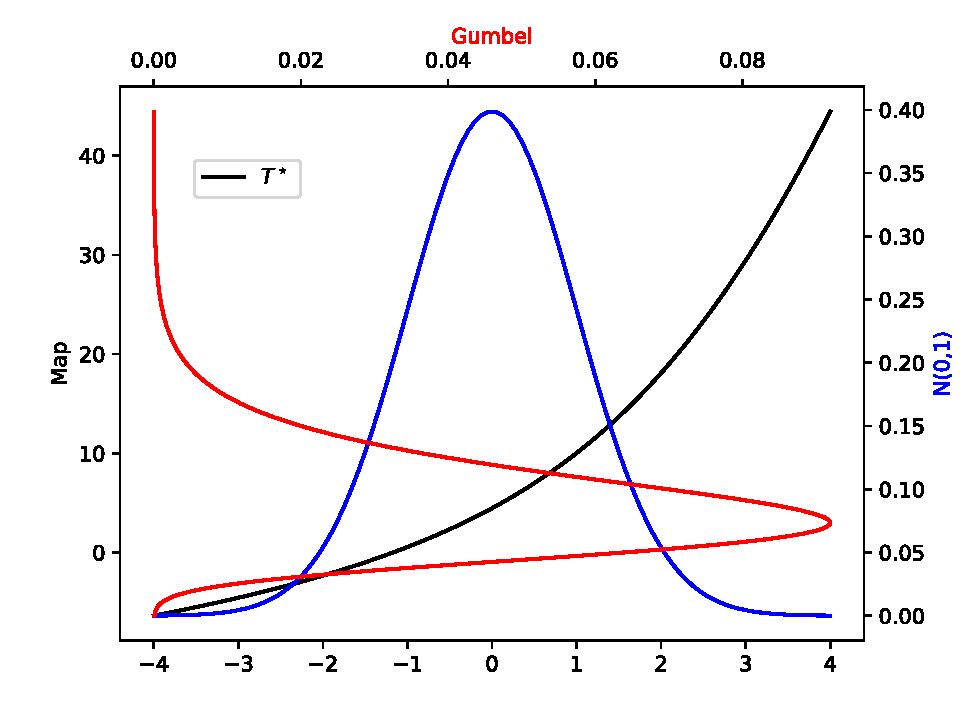
\includegraphics[scale=0.8]{src/figs/GumbelTransportMap.pdf}
\end{figure}


\section{Inference via low-dimensional couplings}
The transport map $T$ can be viewed as a transormation that moves particles : given a collection of samples from $v_{\eta}$ , $T$ rearranges them in accordance with the new distribution $v_{\pi}$

Optimal transprt maps, for instance, define couplings that minimize a particular integrated transport cost expressing the effort required to rearrage samples. In recent years, several other couplings have been proposed for use in statistical problems, e.g.,

\begin{itemize}
\item parametric approximations -- Moselhy, T. and Marzouk, Y. (2012). Bayesian inference with optimal maps. Journal of Computational Physics 231 7815–7850.
\item Knote-Rosenblatt rearrangement-- Rosenblatt, M. (1952). Remarks on a multivariate transformation. The Annals of Mathematical Statistics 470–472
\item coupling induced by ODE flows--- Heng, J., Doucet, A. and Pokern, Y. (2015). Gibbs flow for approximate transport with applications to Bayesian computation. arXiv:1509.08787.
Daum, F. and Huang, J. (2008). Particle flow for nonlinear filters with log-homotopy. In SPIE Defense and Security Symposium 696918–696918. International Society for Optics and Photonics.
Anderes, E. and Coram, M. (2012). A general spline representation for nonparametric and semiparametric density estimates using diffeomorphisms. arXiv:1205.5314.
\end{itemize}

\textbf{Yet the construction, representation, and evaluation of all these maps grows challenging in high dimensions.}

The central contribution of this paper is to \textbf{establish a link between the conditional independence structure of the target measure and the existence of special low dimensional coupling. These couplings are induced by transport maps that are sparse or decomposable.}

\begin{itemize}
\item sparse: A sparse map consists of scalar-valued compnent functions that each depend only a few input variables
\item decomposable map: A decomposable map factorizes as the exact composition of finitely many functions of low effective dimension(i.e, $T = T_1 \circ ... \circ T_l$, where each $T_i$ differs from the identity map only along a subset of its components).
\end{itemize}

The utility of thses results is twofold:
\begin{itemize}
\item First, they make the construction of couplings tractable for a large class of inference problems.
\item Second, they suggest new algorithmic approaches for important classed of statistical models.
\end{itemize}

\subsection{Notation}
\begin{itemize}
\item $f \circ g$: the composition of $f,g$
\item $\partial_k f$ partial derivative of $f$ with respect to its $k$th input variable
\item $x \rightarrow Qx$: linear map
\item $T_{\sharp} v$: pushforward measure given by $v \circ T^{-1}$
\item $T^{-1}(B)$: set-valued preimage of $B$ under T
\item $T^{\sharp}v$: the pullback measure given by $v \circ T$
\item $T_{\sharp} \pi$:
\end{itemize}

\subsection{Triangular transport maps: a building block}





\section{An Optimal Transport Formulation of the Linear Feedback Particle
Filter}
Based on the concept of optimal transportation, a time-stepping optimization procedure is proposed here to obtain a unique optimal control law, denoted as $\mu_t^*$ and $K_t^*$. In this procedure, a finite time interval is divided into discrete time steps $t_0,...,t_n$.
Then a discrete time random process, $S_{t_k}$ is constructed by initializing $S_{t_0}$ according to the initial prior $P(X_0)$, and sequentially evolving $S_{t_k} \rightarrow S_{t_{k+1}}$ at each time-step with a map denoted by $T_k$:
\begin{equation}
S_{t_{k+1}} = T_k(S_{t_k}),  S_0   P(X_0)
\end{equation}

% The map $T_k$ is obtained by solving an optimal transportation problem between the conditional probability distributions at time instants $t_{k}$ and $t_{k+1}$, between $P(X_{t_k}|Z_{t_k})$ and $P(X_{t_{k+1}}|Z_{t_{k+1}})$.


% By construction, $S_{t_k}$ is distributed according to $P(X_{t_k}|Z_{t_k}).


\subsection{Exactness and non-uniqueness}




\section{transportmaps.mit.edu}
\subsection{Bayesian models}
Bayesian models arise naturally in statistical inference problems, where the belief represented by a prior probability distribution
need to be updated according to some observations. We can summarize these models as follows.

Let $G: \mathbb{R}^d \rightarrow \mathbb{R}^{d_z}$ be a map, let $X \in \mathbb{R}^d$ be a random variable with distribution $v_{\rho}$, representing the prior belief on the state of $X$. Let $d \in \mathbb{R}^{d_y}$ be observations of the output of $G$ for some unknown inputs $x \in \mathbb{R}^d$ obtained through the observations. This model for the measurements
\begin{equation}
d = f(G(x),\xi)
\end{equation}
we defin the posterior distribution $v_{\pi}$ by its density
\[
 \pi(x|Y = d) \approx \mu(f^{-1}(G(x),d)) \rho(x) = \mathcal{L}(x) \rho(x)
 \]
 $ \mathcal{L}(x)  $ is the likelihood and $  \rho(x)$ is the prior density.
 \subsubsection{Linear Gaussian model}
 Let us consider here the linear model $G(x) = Gx$ with additive Gaussian noise
 \[
 d = G x + \xi
 \]
 This means that the likelihood is defined as
 \[
\mathcal{L}_d(x) = \mu(d - Gx)
 \]

Let the prior distribution on $X$ be Gaussian, $v_{\rho} \sim \mathcal{N}(m_{\rho},\Sigma_{\rho})$.

\textbf{Feedback particle filter:} The feedback particle filter for linear Gaussian problem is given by


\subsection{Background on optimal transportation}
Let $P_X$ and $P_Y$ be two given probability measures on $\mathbb{R}^d$ with finite second moments. The optimal transportation problem is to minimize
\[
 min_T \quad E[(T(x) - x)^2]
\]
over all maps $T: \mathbb{R}^d \rightarrow \mathbb{R}^d$ such that:
\[
X \sim P_X, \quad T(x) \sim P_Y
\]
If it exists, the minimizer $T^*$, is called the optimal transport map between $P_X$ and $P_Y$. The optimal cost is referred to as $L^2-$Wasserstein distance between $P_X$ and $P_Y$.

\subsubsection{Optimal map between Gaussians}
Suppose $P_X$ and $P_Y$ are Gaussian distributions, $\mathcal{N}(X,\Sigma_X)$ and $\mathcal{N}(Y,\Sigma_Y)$. Then the optimal transport map between $P_X$ and $P_Y$ is given by:
\[
T(x) = Y + F(x - X)
\]
where
\[
F = \Sigma_Y^{\frac{1}{2}}(\Sigma_Y^{\frac{1}{2}} \Sigma_X \Sigma_Y^{\frac{1}{2}})^{-\frac{1}{2}}\Sigma_Y^{\frac{1}{2}}
\]




\section{Classical Monge-Kantorovich problem}
In our simplest exercise we generate two of these random histograms and then try to design a transport plan between them. The concise statement of the problem is
\[
min \left\{Tr M^T Z|Z1 = p,Z^T1 = q \right\}
\]
where $p,q$ are $m$ vectors representing the mass of the histogram bars for the source and destination histograms, respectively. The matrix $M$ represents the distances between the pairs of historgram bars, i.e. $M_{i,j} = |x_i - y_j|$. The trace formulation of the objective is simply the discrete analogue of the continuous formulation
\[
min_{\pi \in \prod(\mu,v)} \int c(x,y)d\pi(x,y)
\]
where $\pi(\mu,v)$ for all borel sets $A$ and $B$.  The matrix $Z$ in the discretized problem playes the role of $\pi$ in the continuous formulation, indicating how much mass is to be transfered from points $x$ to point $y$.

\section{Optimal Transport Filtering with Particle Reweighing in Finance}

Particle flow filter(daum) allows the reduction of the number of particles we need in order to get a tolerable level of errors in the filtering problem. The main idea behind this method is the evolution in homotopy parameter $\lambda$ from prior to the target density. The introduced a particle flow, in which particles are gradually transported without the necessity to randomly sample from any distribution.

The idea of transportation and rewighing mechanism is to transport particles through the sequence of densities that move the least during the synthetic time until they reach the posterior distribution. By regenerating particles according  to their weight at each time step we are able to direct the flow and further minimize the variance of the estimates.

\section{Coupling Particle Filter}
Although the optimal mass transport problem has many desirable properties it
also has drawbacks. Monge’s formulation is a \textcolor{blue}{nonconvex optimization problem} and
the Kantorovich formulation results in \textcolor{blue}{large-scale optimization problems}.
A recent development to address this computational problem builds on adding
an entropic barrier term and solving the resulting optimization problem using the
so called \textcolor{red}{Sinkhorn iterations}.


A coupling of particle filters, given two parameter values $\theta$ and $\tilde{\theta}$, refers to a pair of particle systems, denoted by $(w_t^k,x_t^k)_{k=1}^N$ and $(\tilde{w}_t^k,\tilde{x}_t^k)_{k=1}^N$:
\begin{itemize}
\item marginally,each system has the same distribution as if it was generated by a particle filter
\item the two systems are in some sense correlated
\end{itemize}
In the case of particle filters, the goal is to introduce postive correlations between likelihood estimators $\hat{p}(y_{1:t}|\theta)$ and $\hat{p}(y_{1:t}|\tilde{\theta})$, which improves the performance of score estimators and of MH schemes.

Correlating estimators is a classic Monte Carlo technique for variance reduction, and can often
be achieved by using common random numbers. \textcolor{blue}{Particle filters are randomized algorithms which can be written as a deterministic function of some random variables and a parameter value. However, they are discontinuous functions of their inputs, due to the resampling steps.}

\textcolor{red}{ Our proposed strategy relies on common random numbers for the initialization and propagation steps,
while the resampling step is performed jointly for a pair of particle systems, using ideas inspired
by maximal couplings and optimal transport ideas.}
\subsection{Coupled resampling}
\subsubsection{Common random numbers}
Within particle filters, random variables are used to initialize, to resample and to propagate the
particles. We thus separate the randomness in process-generating variables from
the resampling step, and consider resampling algorithms designed to correlate the particles in both
systems.
\subsubsection{ Coupled resampling and coupled particle filters}
We consider the problem of jointly resampling $(w,x)$ and $(\tilde{w},\tilde{x})$. A joint distribution on $\left\{1,...,N \right\}^2$ is characterized by a matrix $P$ with non-negative entries $P^{ij}$, for $i,j \in \left\{1,...,N \right\}$, that sum to one. The value $P^{ij}$ represents the probability of sampling the pair $(i,j)$. We consider the set $\mathcal{J}(w,\tilde{w})$ of matrices $P$ such that $P \mathbb{1} = w$ and $P^T \mathbb{1} = \tilde{w}$. The choice $P = w \tilde{w}^T$ corresponds to an independent coupling of $w$ and $\tilde{w}$. Sampling from this matrix $P$ is done by sampling $a$ with probabilities $w$ and $\tilde{a}$ with probabilities $\tilde{w}$.


 We now investigate particular choices of matrices $P \in \mathcal{J}(w,\tilde{w})$ with the aim of correlating a pair of particle systems.
\subsubsection{Transport resampling}
Intuitively, we want to choose  $P \in \mathcal{J}(w,\tilde{w})$ such that, upon sampling ancestors from $P$, the resampled particles are as similar as possible between the two systems.

The expected distance between the resampled particles $x^a$ and $\tilde{x}^{\tilde{a}}$, conditional upon $(w,x)$ and $(\tilde{w},\tilde{x})$, is given by $\sum_{i=1}^N \sum_{j=1^N} P^{ij}d(x^i,\tilde{x}^j)$. Denote by $D$ the distance matrix with entries $D^{ij} = d(x^i,\tilde{x}^j)$. The optimal transport problem considers a matrix $P^*$ that minimizes the expected distance over all $P \in \mathcal{J}(w,\tilde{w})$.


\section{Inference via low-dimensional couplings}

\subsection{Triangular transport maps: a building block}
An essential feature of the trangular transport map is its anisotropic dependence on the input variables. That is, even though each component of the transport map does not depend on all $n$ inputs, the map is still capable of coupling arbitrary probability distribution.

All these approaches face a fundamental challenge: the transport map is a function from $\mathbb{R}^n$ on itself, and in high dimensions the representation and approximation of such functions becomes increasingly intractable.

\subsection{Markov networks}
Let $\mathbf{Z} = (Z_1,...,Z_n)$ be a collection of random variables with law $v_{\pi}$ and density $\pi$. We can represent a list of conditional independences satisfied by $\mathbf{Z}$-the so-called Markov properties-using a simple undirected graph $\mathcal{G} = (\mathcal{V},\mathcal{E})$, where each node $k \in \mathcal{V}$ is associated with a distinct random variable, $Z_k$, and where the edges in $\mathcal{E}$ encode a specific notion of probabilisitic interaction among these random variables.
\subsection{Sparisty of triangular transport maps}
A sparse map is a multivariate function where each comonent does not depend on all its input variables.
\subsubsection{Sparisity bounds}



\section{local couplings filter}
The idear of local couplings filter is a generalization of the EnKF phiosophy, and can be synthesized as follows: we seek to transorm the forecast ensemble into samples from the filtering distribution by means of a sequence of local, low-dimensional, and possibly nonlinear deterministic couplings.

We have a coolection of random variables, $Z = (Z_1,...,Z_n)$ and $Y$. We should think of $Z$ as a random variable on $\mathcal{R}^n$ distributed according to the forecast distribution at a certain time $t$, whereas we can think of $Y$ as a random variable corresponding to the observed data at the same assimilation time.

\subsection{local assimilation}
First, we need sample from $\pi_{Z_1|Y}$
\end{CJK}
\end{document}